%!TEX root = ../main.tex
\subsection{Implementing CAN utilizing XCanPs}\label{sec:methods_to_implement_can}

\mikkel{DONE:move axi can to analysis.}
\mikkel{move assymetric multiprocesssing to future work}
\mikkel{ move bare metal first}
\mikkel{split from linux part.}
\martin{The can controllers do not have anything to do with xilinux. Does Xilinux provide drivers for the can controllers on the zynq? CAN controllers vs CAN drivers Issue - Some things rephrased.}

This section includes the process that was followed to enable the CAN controller drivers.
The purpose of this was to gain access to the controllers from Linux.
Using this operating system was necessary for using the required USB interfaces, logging the data into files as well as utilizing the network tools to establish an ad-hoc network.
The steps for this were to modify certain files related to the kernel configurations and the device tree settings.

\subsubsection*{Enabling the CAN Controller Drivers}

According to Xilinx documentation, the process for enabling the CAN controllers on the Zynq7 Processing System, the Linux CAN driver guide \cite{Xilinx_wiki_Linux_CAN_driver} was needed to be followed.
Specifically, the Kconfig file under the path \ref{code:can_kconfig_pathfile} needed to be configured.
The entry at line 128 was changed as seen in code \ref{code:can_kconfig_contents_line128}.
Originally, lines 130 and 131 were as seen in code \ref{code:can_kconfig_original_line130}.

\begin{lstlisting}[caption={CAN Kconfig pathfile.},numbers=none,label=code:can_kconfig_pathfile]
/usr/src/kernels/3.12.0-xillinux-1.3/drivers/net/can
\end{lstlisting}

\begin{lstlisting}[firstnumber=128,caption={Kconfig file contents from line 128.},label={code:can_kconfig_contents_line128}]
config CAN_XILINXCAN
	tristate "Xilinx(*@ @*)CAN"
	depends on NET [=y] && CAN_DEV [=y] && CAN [=y] && 
        (ARCH_ZYNQ || MICROBLAZE [=y])
	default y
\end{lstlisting}

\begin{lstlisting}[firstnumber=130,caption={Original content of lines 130 and 131.},label={code:can_kconfig_original_line130}]
	depends on CAN && (ARCH_ZYNQ || MICROBLAZE)
	default n
\end{lstlisting}

The next step of the process was the modification of the device tree settings file, requiring an entry for the CAN PS to be inserted.
The necessary file was located under the boot folder named as seen in \ref{code:dts_file_zybo}.
The modifications can be seen in code \ref{code:dts_changes_zybo} for can controllers as well as for the AXI CAN core.

\begin{lstlisting}[numbers=none,caption={Device tree settings file and its path.},label={code:dts_file_zybo}]
/boot/xillinux-1.3-zybo.dts
\end{lstlisting}
\catalin{Double quotes are problem here as well. FIX THEM WHENEVER}
\begin{lstlisting}[caption={Device tree settings changes.},label={code:dts_changes_zybo}]
zynq_can_0: can@e0008000 {
        compatible = xlnx,zynq-can-1.0;
        clocks = <&clkc 19>, <&clkc 36>;
        clock-names = can_clk, pclk;
        reg = <0xe0008000 0x1000>;
        interrupts = <0 28 4>;
        interrupt-parent = <&intc>;
        tx-fifo-depth = <0x40>;
        rx-fifo-depth = <0x40>;
    };
axi_can_0: axi-can@40000000 {
        compatible = xlnx,axi-can-1.00.a;
        clocks = <&clkc 0>, <&clkc 1>;
        clock-names = can_clk,s_axi_aclk;
        reg = <0x40000000 0x10000>;
        interrupt-parent = <&intc>;
        interrupts = <0 59 1>;
        tx-fifo-depth = <0x40>;
        rx-fifo-depth = <0x40>;
        };
\end{lstlisting}

Unfortunately, the above steps did not enable the drivers successfully.
After the changes, the CAN devices were still not visible in Linux and thus, connection to the CAN network was not feasible.

\mikkel{Maybe you can provide some thoughts about the problem.
Maybe also some words about the patching Xilinx-Digilent etc.}
As was previously mentioned, the implementation was unsuccessful.
At the time, the research done on this topic did not lead to successfully enabling the drivers.

%The architecture can be seen in figure \ref{fig:CAN_Arch_with_AXI_CAN}.

%\begin{figure}[h!]
%	\centering
%	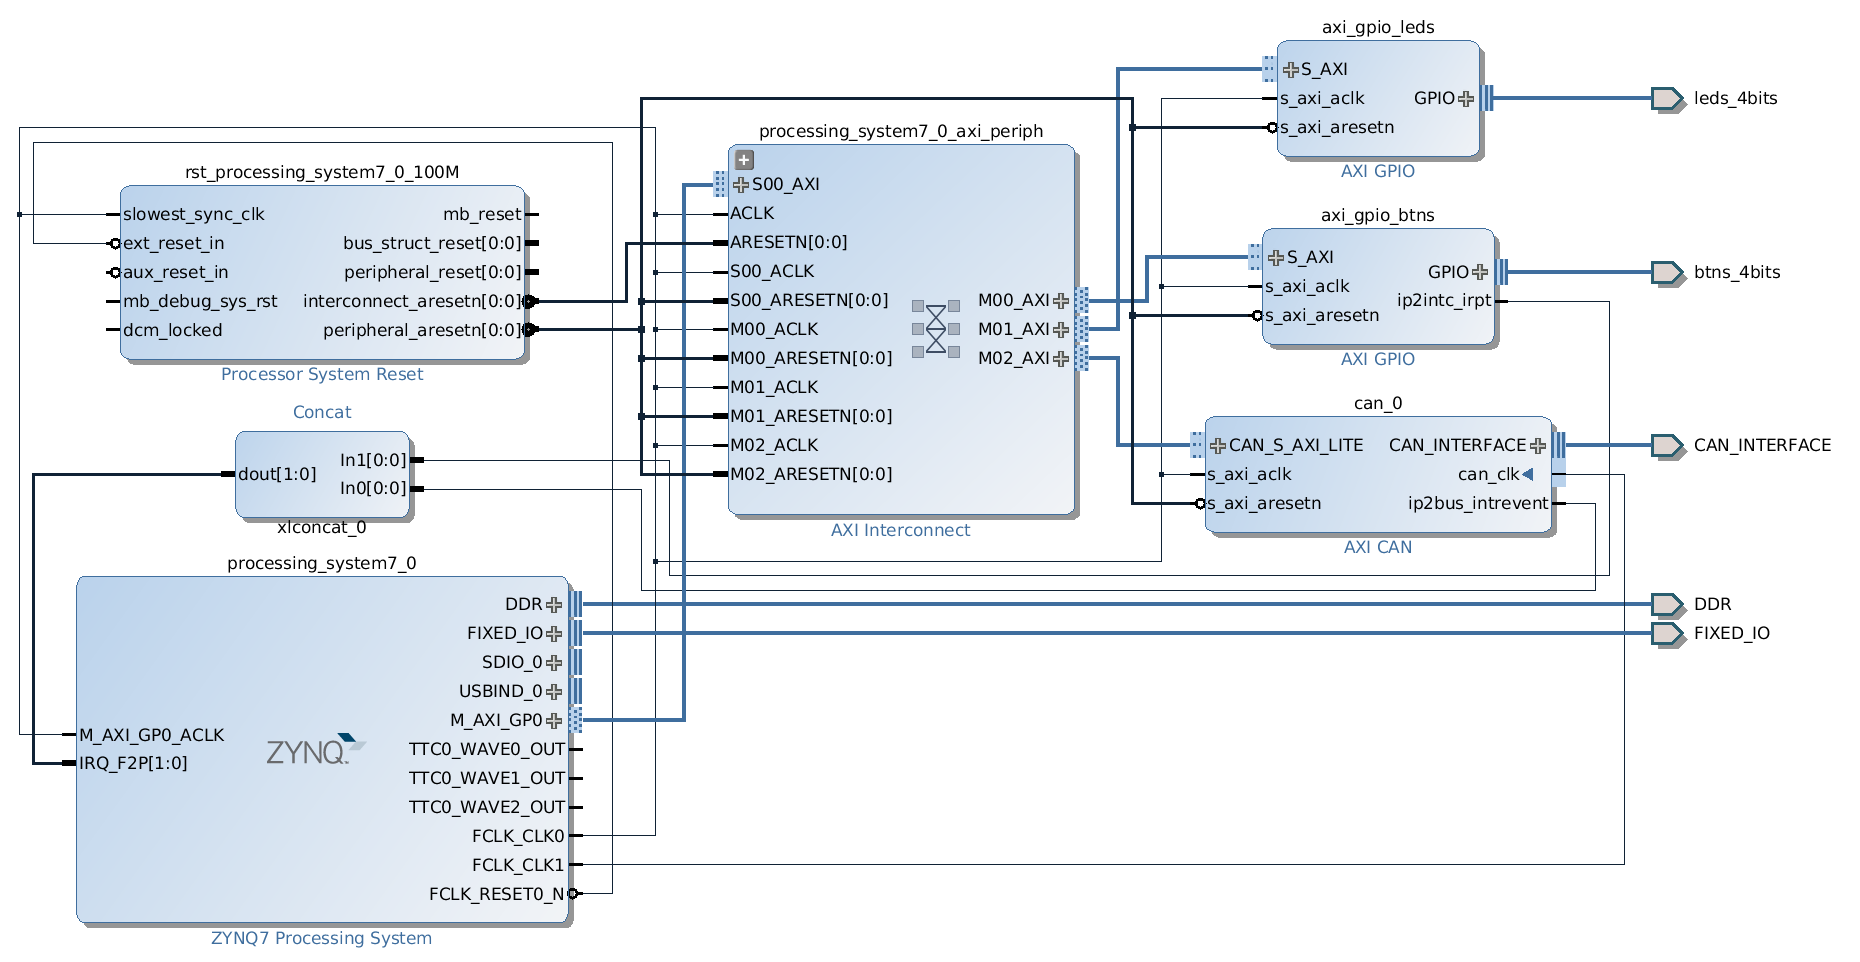
\includegraphics[width = 1.2\linewidth]{graphics/Zybo_Arch_with_AXI_CAN.png}
%	\caption{Block diagram featuring the architecture in Vivado with the AXI CAN core.}
%	\label{fig:CAN_Arch_with_AXI_CAN}
%\end{figure}
